\PassOptionsToPackage{unicode=true}{hyperref} % options for packages loaded elsewhere
\PassOptionsToPackage{hyphens}{url}
%
\documentclass[ignorenonframetext,]{beamer}
\usepackage{pgfpages}
\setbeamertemplate{caption}[numbered]
\setbeamertemplate{caption label separator}{: }
\setbeamercolor{caption name}{fg=normal text.fg}
\beamertemplatenavigationsymbolsempty
% Prevent slide breaks in the middle of a paragraph:
\widowpenalties 1 10000
\raggedbottom
\setbeamertemplate{part page}{
\centering
\begin{beamercolorbox}[sep=16pt,center]{part title}
  \usebeamerfont{part title}\insertpart\par
\end{beamercolorbox}
}
\setbeamertemplate{section page}{
\centering
\begin{beamercolorbox}[sep=12pt,center]{part title}
  \usebeamerfont{section title}\insertsection\par
\end{beamercolorbox}
}
\setbeamertemplate{subsection page}{
\centering
\begin{beamercolorbox}[sep=8pt,center]{part title}
  \usebeamerfont{subsection title}\insertsubsection\par
\end{beamercolorbox}
}
\AtBeginPart{
  \frame{\partpage}
}
\AtBeginSection{
  \ifbibliography
  \else
    \frame{\sectionpage}
  \fi
}
\AtBeginSubsection{
  \frame{\subsectionpage}
}
\usepackage{lmodern}
\usepackage{amssymb,amsmath}
\usepackage{ifxetex,ifluatex}
\usepackage{fixltx2e} % provides \textsubscript
\ifnum 0\ifxetex 1\fi\ifluatex 1\fi=0 % if pdftex
  \usepackage[T1]{fontenc}
  \usepackage[utf8]{inputenc}
  \usepackage{textcomp} % provides euro and other symbols
\else % if luatex or xelatex
  \usepackage{unicode-math}
  \defaultfontfeatures{Ligatures=TeX,Scale=MatchLowercase}
\fi
\usecolortheme{beaver}
% use upquote if available, for straight quotes in verbatim environments
\IfFileExists{upquote.sty}{\usepackage{upquote}}{}
% use microtype if available
\IfFileExists{microtype.sty}{%
\usepackage[]{microtype}
\UseMicrotypeSet[protrusion]{basicmath} % disable protrusion for tt fonts
}{}
\IfFileExists{parskip.sty}{%
\usepackage{parskip}
}{% else
\setlength{\parindent}{0pt}
\setlength{\parskip}{6pt plus 2pt minus 1pt}
}
\usepackage{hyperref}
\hypersetup{
            pdftitle={Manejo de datos en R (II)},
            pdfauthor={Introducción a la Línea de Comandos para Análisis Bioinformáticos},
            pdfborder={0 0 0},
            breaklinks=true}
\urlstyle{same}  % don't use monospace font for urls
\newif\ifbibliography
\usepackage{color}
\usepackage{fancyvrb}
\newcommand{\VerbBar}{|}
\newcommand{\VERB}{\Verb[commandchars=\\\{\}]}
\DefineVerbatimEnvironment{Highlighting}{Verbatim}{commandchars=\\\{\}}
% Add ',fontsize=\small' for more characters per line
\usepackage{framed}
\definecolor{shadecolor}{RGB}{248,248,248}
\newenvironment{Shaded}{\begin{snugshade}}{\end{snugshade}}
\newcommand{\AlertTok}[1]{\textcolor[rgb]{0.94,0.16,0.16}{#1}}
\newcommand{\AnnotationTok}[1]{\textcolor[rgb]{0.56,0.35,0.01}{\textbf{\textit{#1}}}}
\newcommand{\AttributeTok}[1]{\textcolor[rgb]{0.77,0.63,0.00}{#1}}
\newcommand{\BaseNTok}[1]{\textcolor[rgb]{0.00,0.00,0.81}{#1}}
\newcommand{\BuiltInTok}[1]{#1}
\newcommand{\CharTok}[1]{\textcolor[rgb]{0.31,0.60,0.02}{#1}}
\newcommand{\CommentTok}[1]{\textcolor[rgb]{0.56,0.35,0.01}{\textit{#1}}}
\newcommand{\CommentVarTok}[1]{\textcolor[rgb]{0.56,0.35,0.01}{\textbf{\textit{#1}}}}
\newcommand{\ConstantTok}[1]{\textcolor[rgb]{0.00,0.00,0.00}{#1}}
\newcommand{\ControlFlowTok}[1]{\textcolor[rgb]{0.13,0.29,0.53}{\textbf{#1}}}
\newcommand{\DataTypeTok}[1]{\textcolor[rgb]{0.13,0.29,0.53}{#1}}
\newcommand{\DecValTok}[1]{\textcolor[rgb]{0.00,0.00,0.81}{#1}}
\newcommand{\DocumentationTok}[1]{\textcolor[rgb]{0.56,0.35,0.01}{\textbf{\textit{#1}}}}
\newcommand{\ErrorTok}[1]{\textcolor[rgb]{0.64,0.00,0.00}{\textbf{#1}}}
\newcommand{\ExtensionTok}[1]{#1}
\newcommand{\FloatTok}[1]{\textcolor[rgb]{0.00,0.00,0.81}{#1}}
\newcommand{\FunctionTok}[1]{\textcolor[rgb]{0.00,0.00,0.00}{#1}}
\newcommand{\ImportTok}[1]{#1}
\newcommand{\InformationTok}[1]{\textcolor[rgb]{0.56,0.35,0.01}{\textbf{\textit{#1}}}}
\newcommand{\KeywordTok}[1]{\textcolor[rgb]{0.13,0.29,0.53}{\textbf{#1}}}
\newcommand{\NormalTok}[1]{#1}
\newcommand{\OperatorTok}[1]{\textcolor[rgb]{0.81,0.36,0.00}{\textbf{#1}}}
\newcommand{\OtherTok}[1]{\textcolor[rgb]{0.56,0.35,0.01}{#1}}
\newcommand{\PreprocessorTok}[1]{\textcolor[rgb]{0.56,0.35,0.01}{\textit{#1}}}
\newcommand{\RegionMarkerTok}[1]{#1}
\newcommand{\SpecialCharTok}[1]{\textcolor[rgb]{0.00,0.00,0.00}{#1}}
\newcommand{\SpecialStringTok}[1]{\textcolor[rgb]{0.31,0.60,0.02}{#1}}
\newcommand{\StringTok}[1]{\textcolor[rgb]{0.31,0.60,0.02}{#1}}
\newcommand{\VariableTok}[1]{\textcolor[rgb]{0.00,0.00,0.00}{#1}}
\newcommand{\VerbatimStringTok}[1]{\textcolor[rgb]{0.31,0.60,0.02}{#1}}
\newcommand{\WarningTok}[1]{\textcolor[rgb]{0.56,0.35,0.01}{\textbf{\textit{#1}}}}
\usepackage{graphicx,grffile}
\makeatletter
\def\maxwidth{\ifdim\Gin@nat@width>\linewidth\linewidth\else\Gin@nat@width\fi}
\def\maxheight{\ifdim\Gin@nat@height>\textheight\textheight\else\Gin@nat@height\fi}
\makeatother
% Scale images if necessary, so that they will not overflow the page
% margins by default, and it is still possible to overwrite the defaults
% using explicit options in \includegraphics[width, height, ...]{}
\setkeys{Gin}{width=\maxwidth,height=\maxheight,keepaspectratio}
\setlength{\emergencystretch}{3em}  % prevent overfull lines
\providecommand{\tightlist}{%
  \setlength{\itemsep}{0pt}\setlength{\parskip}{0pt}}
\setcounter{secnumdepth}{0}

% set default figure placement to htbp
\makeatletter
\def\fps@figure{htbp}
\makeatother

\usepackage{tikz}
\usepackage{graphicx}
\usetikzlibrary{calc}
\usepackage{pgfplots}
\usepackage{environ}
\useoutertheme{miniframes}
\useinnertheme{circles}

\title{Manejo de datos en R (II)}
\author{Introducción a la Línea de Comandos para Análisis Bioinformáticos}
\date{03 de Marzo, 2020}

\begin{document}
\frame{\titlepage}

\begin{frame}{Análisis reproducible}
\protect\hypertarget{anuxe1lisis-reproducible}{}

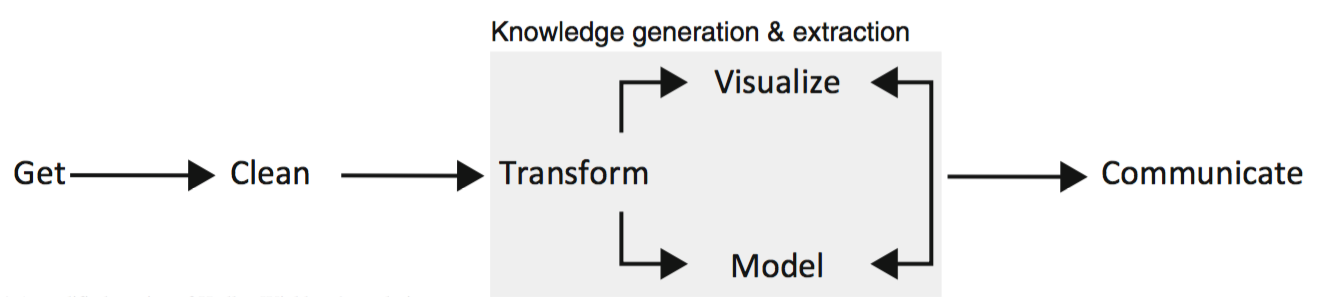
\includegraphics{analytic_process.png}

\end{frame}

\begin{frame}{Operaciones sobre datos}
\protect\hypertarget{operaciones-sobre-datos}{}

\begin{itemize}
\tightlist
\item
  Cargar datos \emph{crudos}/Guardar datos finales y tablas de interés.
\item
  Filtrar datos (con criterio).
\item
  Unir datos que vienen de diferentes fuentes, referentes a un mismo
  conjunto estudiado.
\item
  Hacer modificaciones: crear \emph{tags}, correcciones ortográficas,
  filas y columnas de tablas, etc\ldots{}
\item
  Generar nuevos datos: obtener promedios, medianas, aplicar funciones
  de librerías.
\item
  Dejar anotado y reportar lo hecho.
\end{itemize}

\end{frame}

\begin{frame}{}
\protect\hypertarget{section}{}

\begin{tikzpicture}[remember picture,overlay]
  \node[anchor=south west,inner sep=0pt] at ($(current page.south west)+(0cm,7.8cm)$) {
     
\includegraphics[width=1.5cm]{tidyverse.png}
  };
\end{tikzpicture}

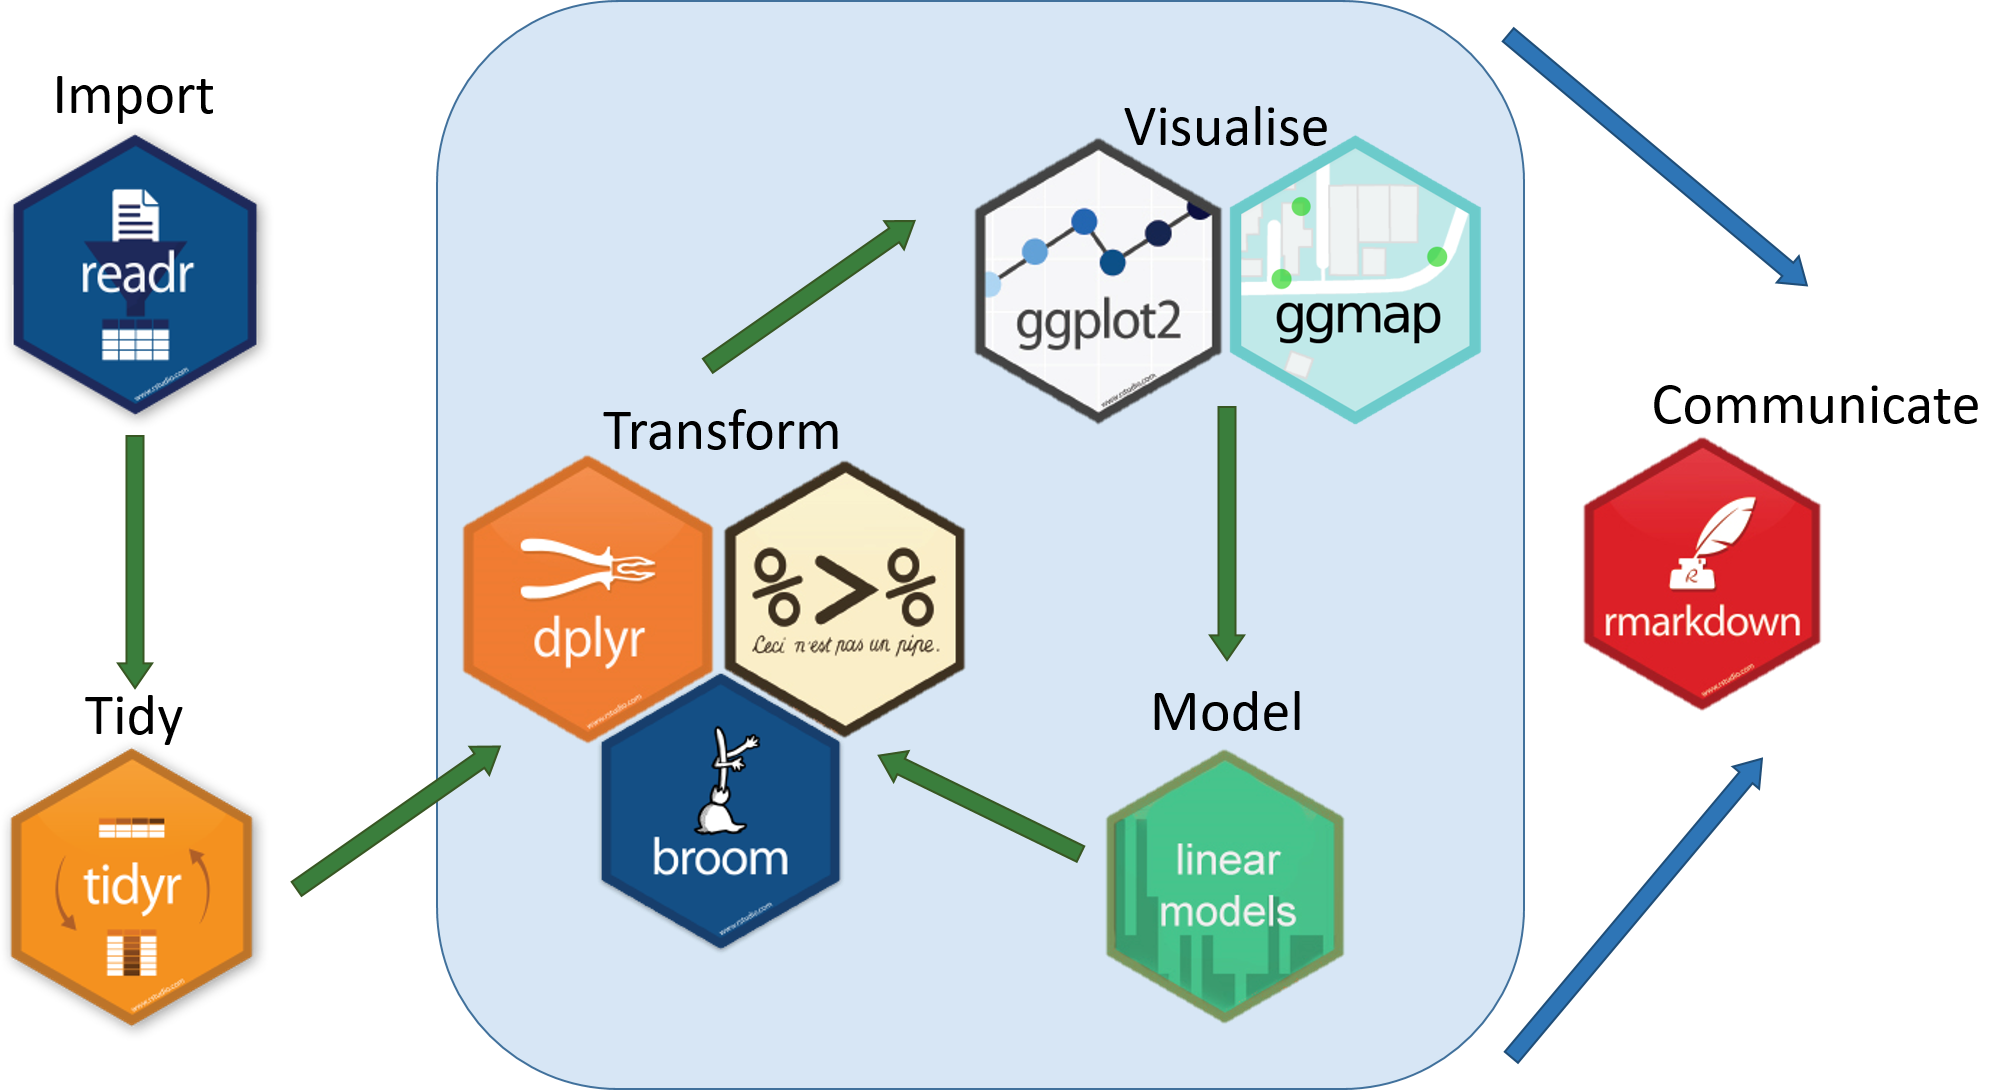
\includegraphics{tidyverse_packages.png}

\end{frame}

\begin{frame}[fragile]{}
\protect\hypertarget{section-1}{}

\begin{tikzpicture}[remember picture,overlay]
  \node[anchor=south west,inner sep=0pt] at ($(current page.south west)+(0cm,7.8cm)$) {
     
\includegraphics[width=1.5cm]{tibbles.png}
  };
\end{tikzpicture}

\small

\begin{Shaded}
\begin{Highlighting}[]
\KeywordTok{library}\NormalTok{(tibble)}

\KeywordTok{as_tibble}\NormalTok{(iris)}
\end{Highlighting}
\end{Shaded}

\begin{verbatim}
## # A tibble: 150 x 5
##    Sepal.Length Sepal.Width Petal.Length Petal.Width Species
##           <dbl>       <dbl>        <dbl>       <dbl> <fct>  
##  1          5.1         3.5          1.4         0.2 setosa 
##  2          4.9         3            1.4         0.2 setosa 
##  3          4.7         3.2          1.3         0.2 setosa 
##  4          4.6         3.1          1.5         0.2 setosa 
##  5          5           3.6          1.4         0.2 setosa 
##  6          5.4         3.9          1.7         0.4 setosa 
##  7          4.6         3.4          1.4         0.3 setosa 
##  8          5           3.4          1.5         0.2 setosa 
##  9          4.4         2.9          1.4         0.2 setosa 
## 10          4.9         3.1          1.5         0.1 setosa 
## # ... with 140 more rows
\end{verbatim}

\normalsize

\end{frame}

\begin{frame}{}
\protect\hypertarget{section-2}{}

\begin{tikzpicture}[remember picture,overlay]
  \node[anchor=south west,inner sep=0pt] at ($(current page.south west)+(0cm,7.8cm)$) {
     
\includegraphics[width=1.5cm]{dplyr.png}
  };
\end{tikzpicture}


\includegraphics{filtro_filas.png}


\includegraphics{filtro_columna.png}

\end{frame}

\begin{frame}{}
\protect\hypertarget{section-3}{}

\begin{tikzpicture}[remember picture,overlay]
  \node[anchor=south west,inner sep=0pt] at ($(current page.south west)+(0cm,7.8cm)$) {
     
\includegraphics[width=1.5cm]{dplyr.png}
  };
\end{tikzpicture}

\begin{center}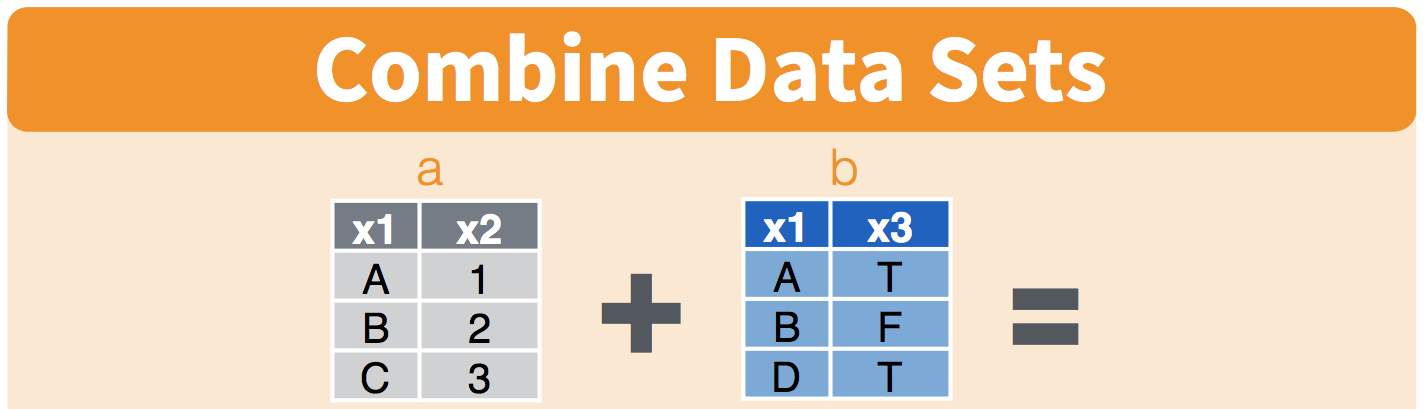
\includegraphics[width=0.5\linewidth]{combinando_dplyr} \end{center}

\begin{center}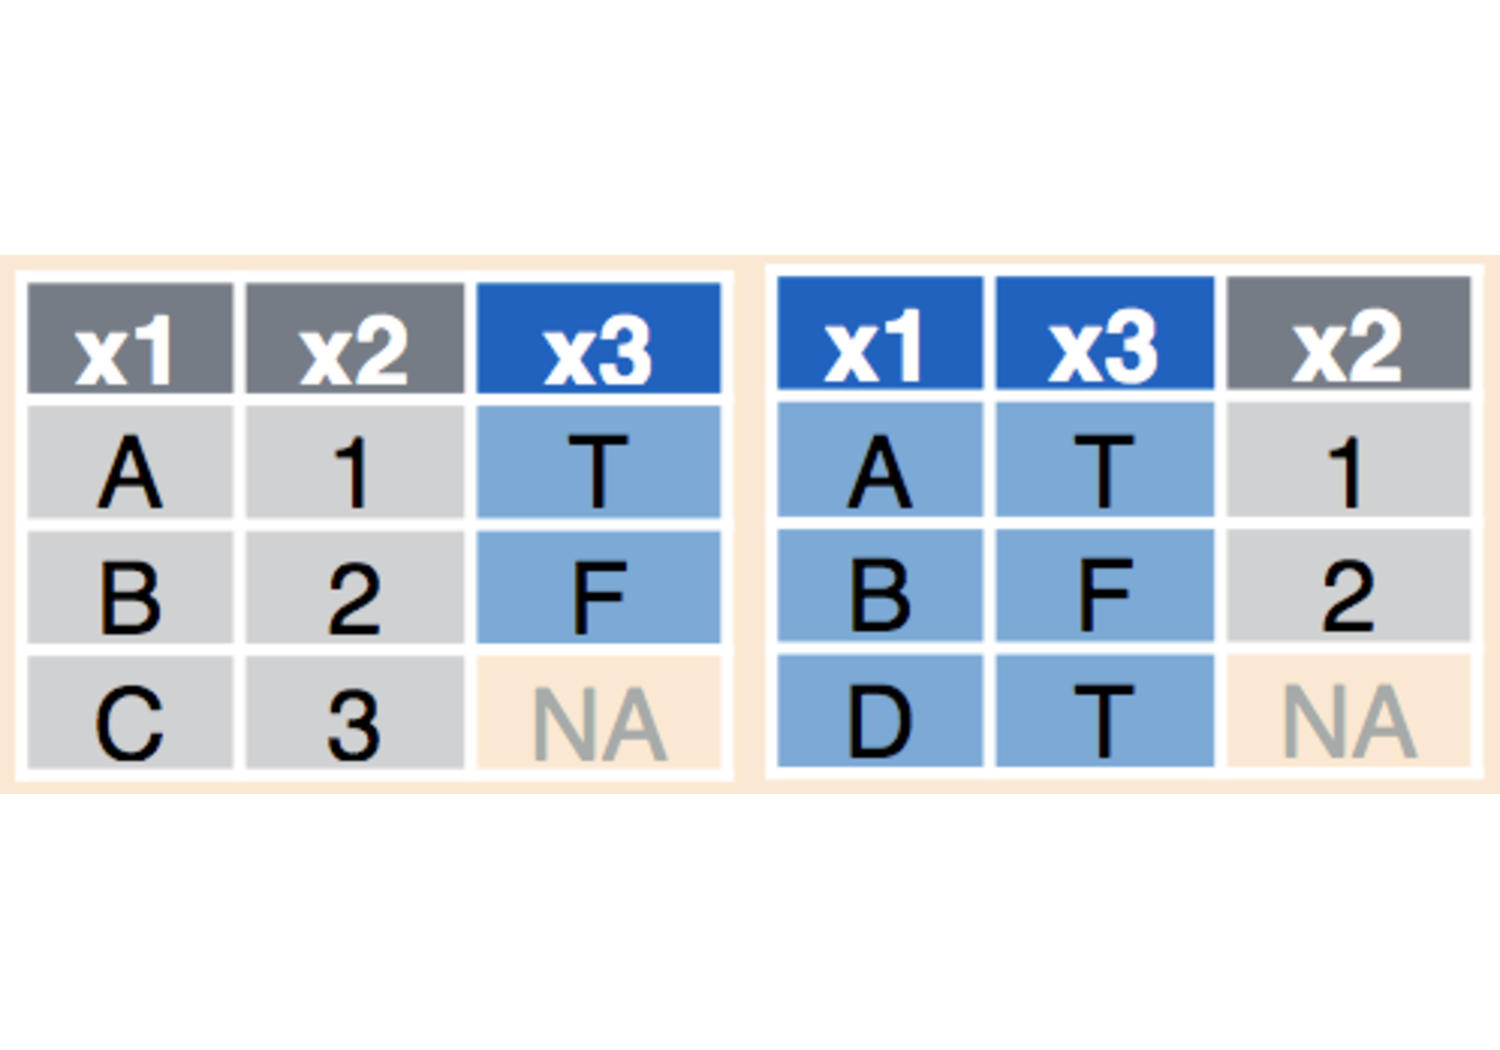
\includegraphics[width=0.4\linewidth]{claseIntro_practico12_final_files/figure-beamer/unnamed-chunk-13-1} \end{center}

\begin{center}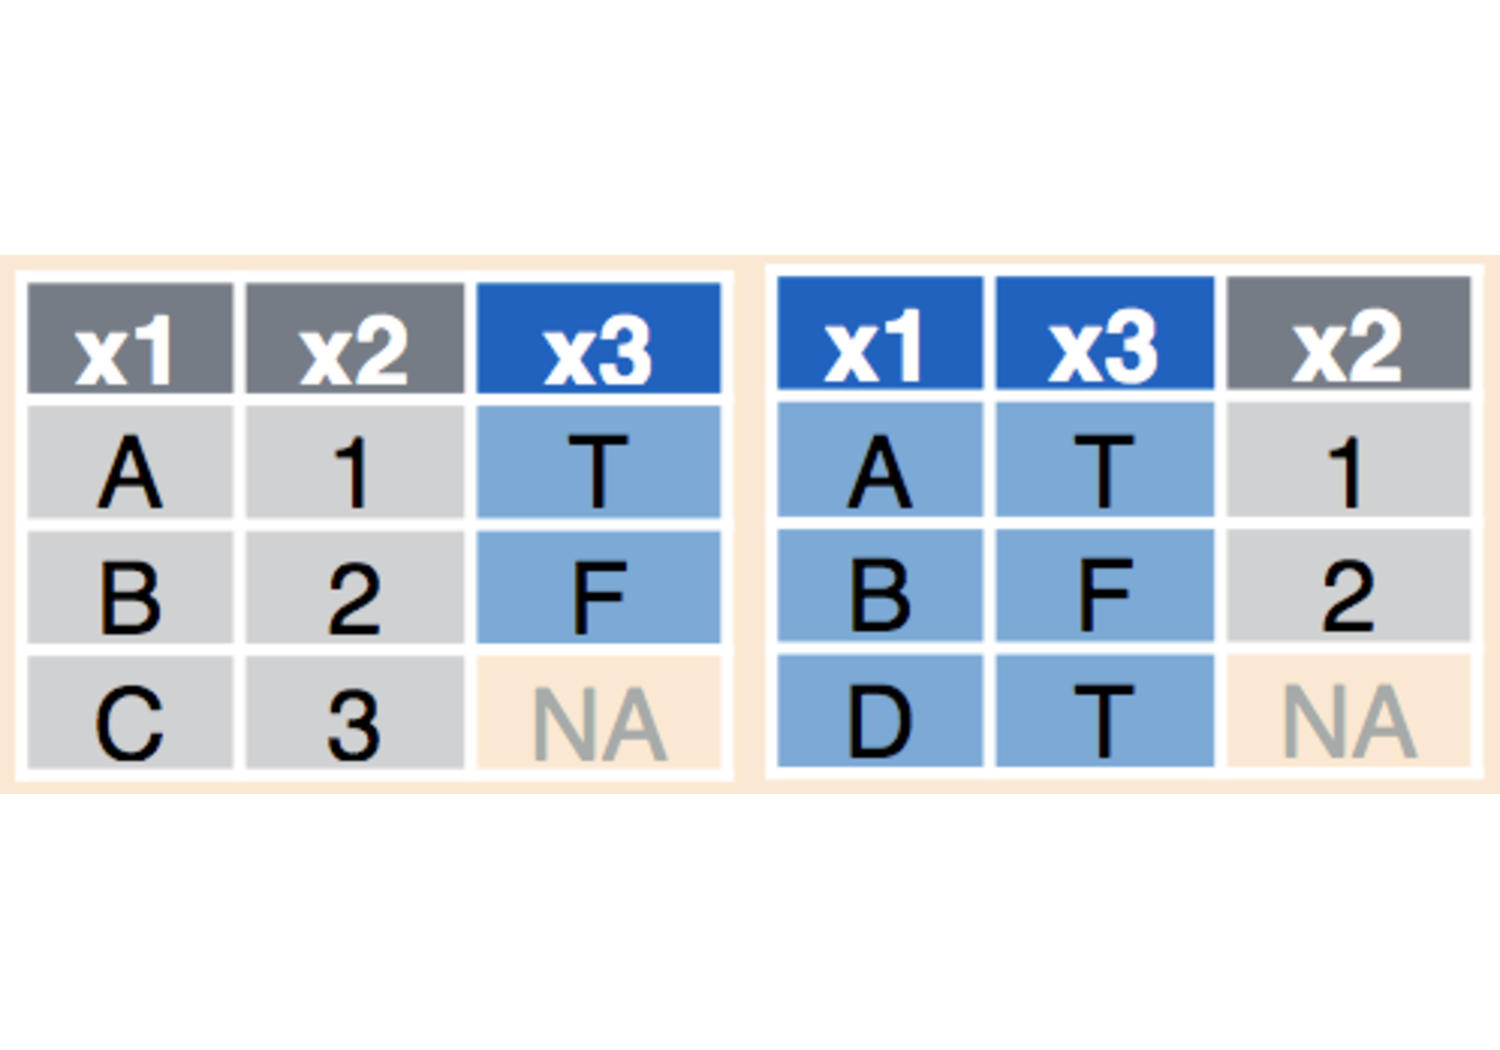
\includegraphics[width=0.4\linewidth]{claseIntro_practico12_final_files/figure-beamer/unnamed-chunk-14-1} \end{center}

\end{frame}

\begin{frame}{}
\protect\hypertarget{section-4}{}

\begin{tikzpicture}[remember picture,overlay]
  \node[anchor=south west,inner sep=0pt] at ($(current page.south west)+(0cm,7.8cm)$) {
     
\includegraphics[width=1.5cm]{dplyr.png}
  };
\end{tikzpicture}

\begin{itemize}
\tightlist
\item
  Con dplyr es posible dividir el análisis de la tabla según una
  columna, y luego operar sobre en base a esto
\end{itemize}

\begin{center}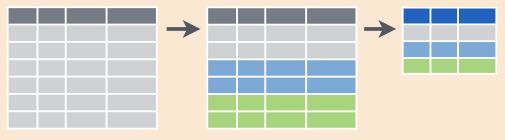
\includegraphics[width=1\linewidth]{dplyr_groupBy_summarise} \end{center}

\end{frame}

\begin{frame}{Tablas\ldots{} todas dan igual?}
\protect\hypertarget{tablas-todas-dan-igual}{}

\begin{center}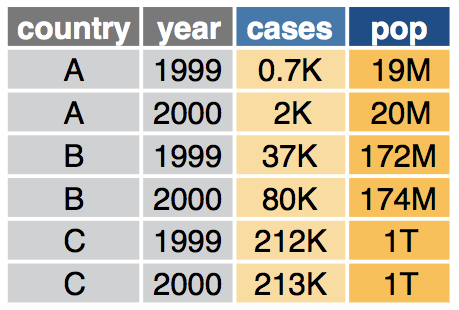
\includegraphics[width=0.7\linewidth]{data_wide} \end{center}

\end{frame}

\begin{frame}{Tablas\ldots{} todas dan igual?}
\protect\hypertarget{tablas-todas-dan-igual-1}{}

\begin{center}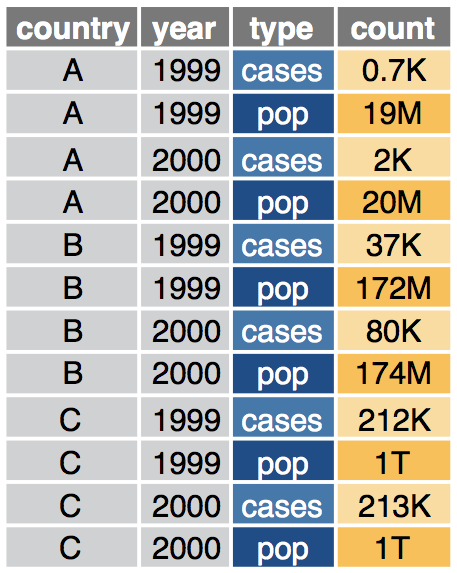
\includegraphics[width=0.55\linewidth]{data_long} \end{center}

\end{frame}

\begin{frame}{}
\protect\hypertarget{section-5}{}

\begin{tikzpicture}[remember picture,overlay]
  \node[anchor=south west,inner sep=0pt] at ($(current page.south west)+(0cm,7.8cm)$) {
     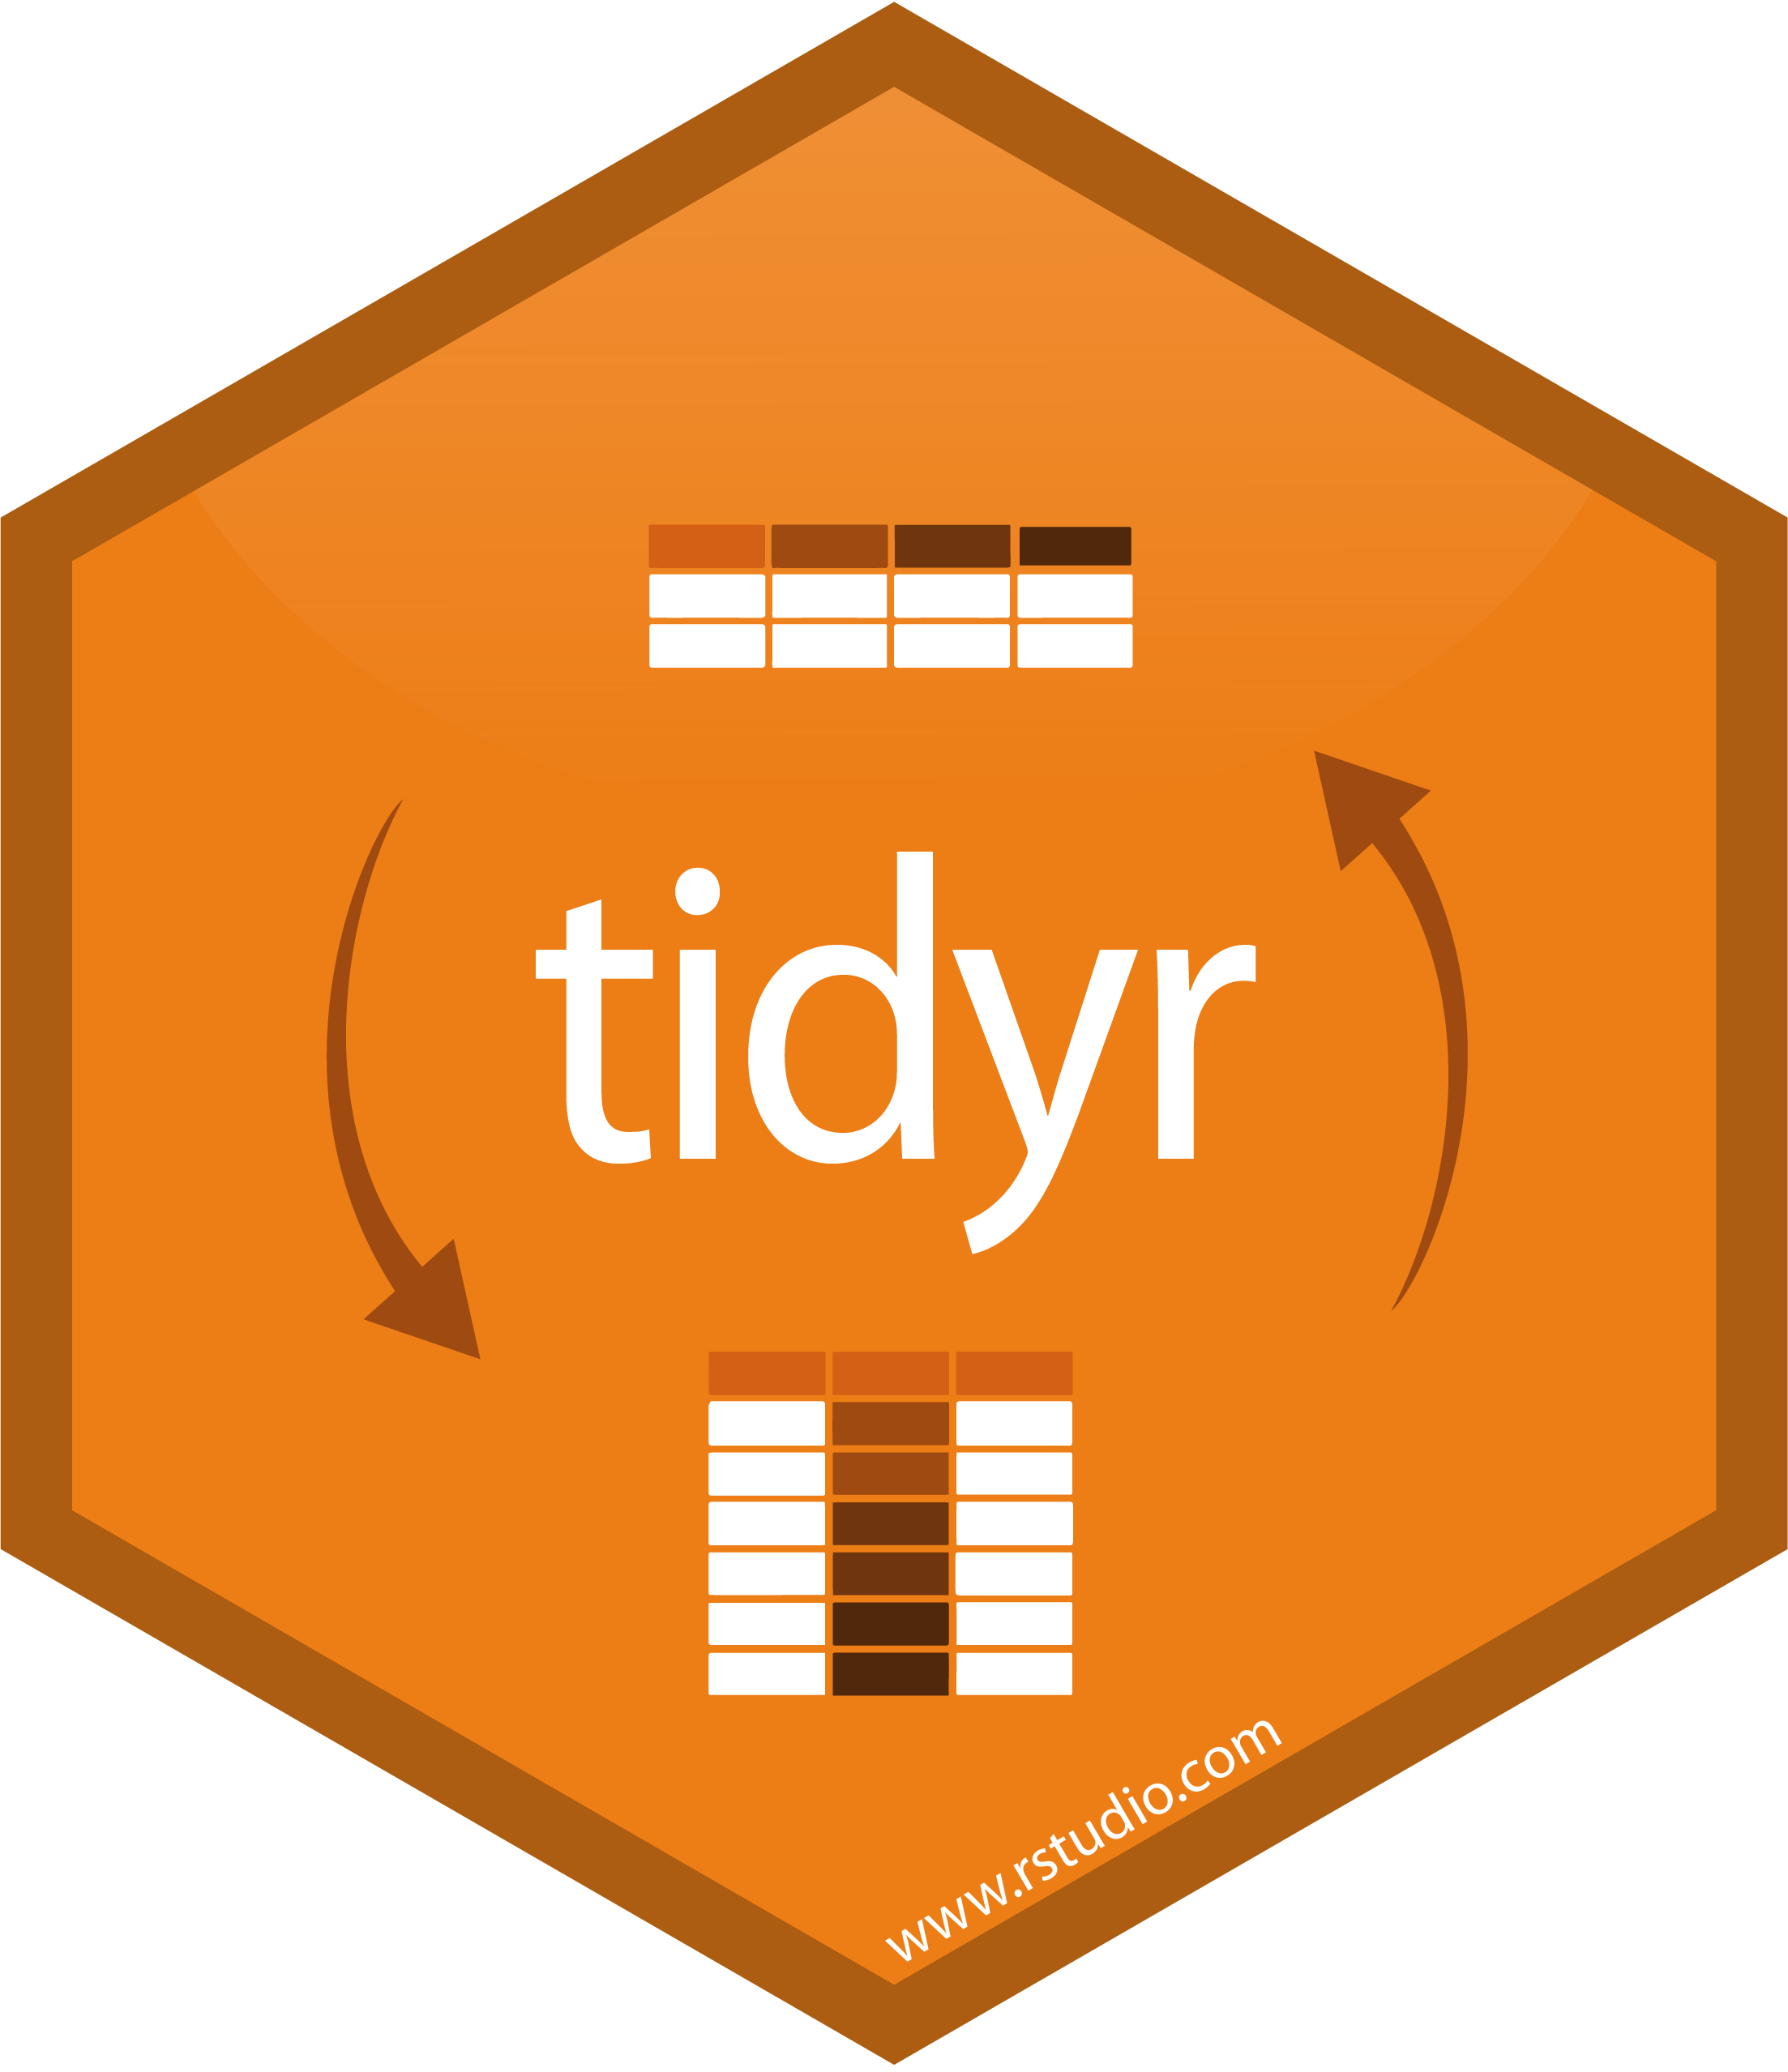
\includegraphics[width=1.5cm]{tidyr.png}
  };
\end{tikzpicture}

\begin{itemize}
\tightlist
\item
  Podemos llevar una tabla a formato alargado
\end{itemize}

\begin{flushright}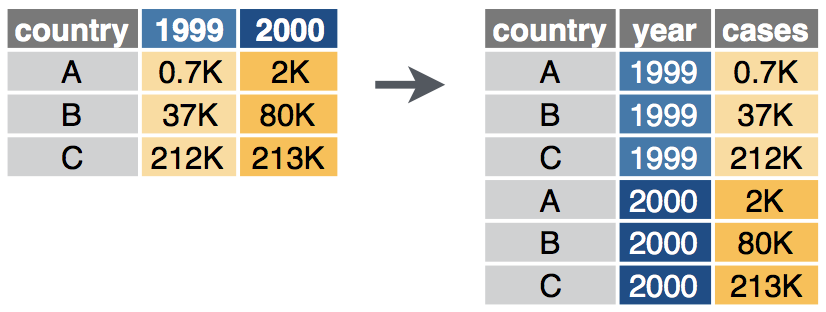
\includegraphics{pivot_longer_detailed} \end{flushright}

\end{frame}

\begin{frame}{}
\protect\hypertarget{section-6}{}

\begin{tikzpicture}[remember picture,overlay]
  \node[anchor=south west,inner sep=0pt] at ($(current page.south west)+(0cm,7.8cm)$) {
     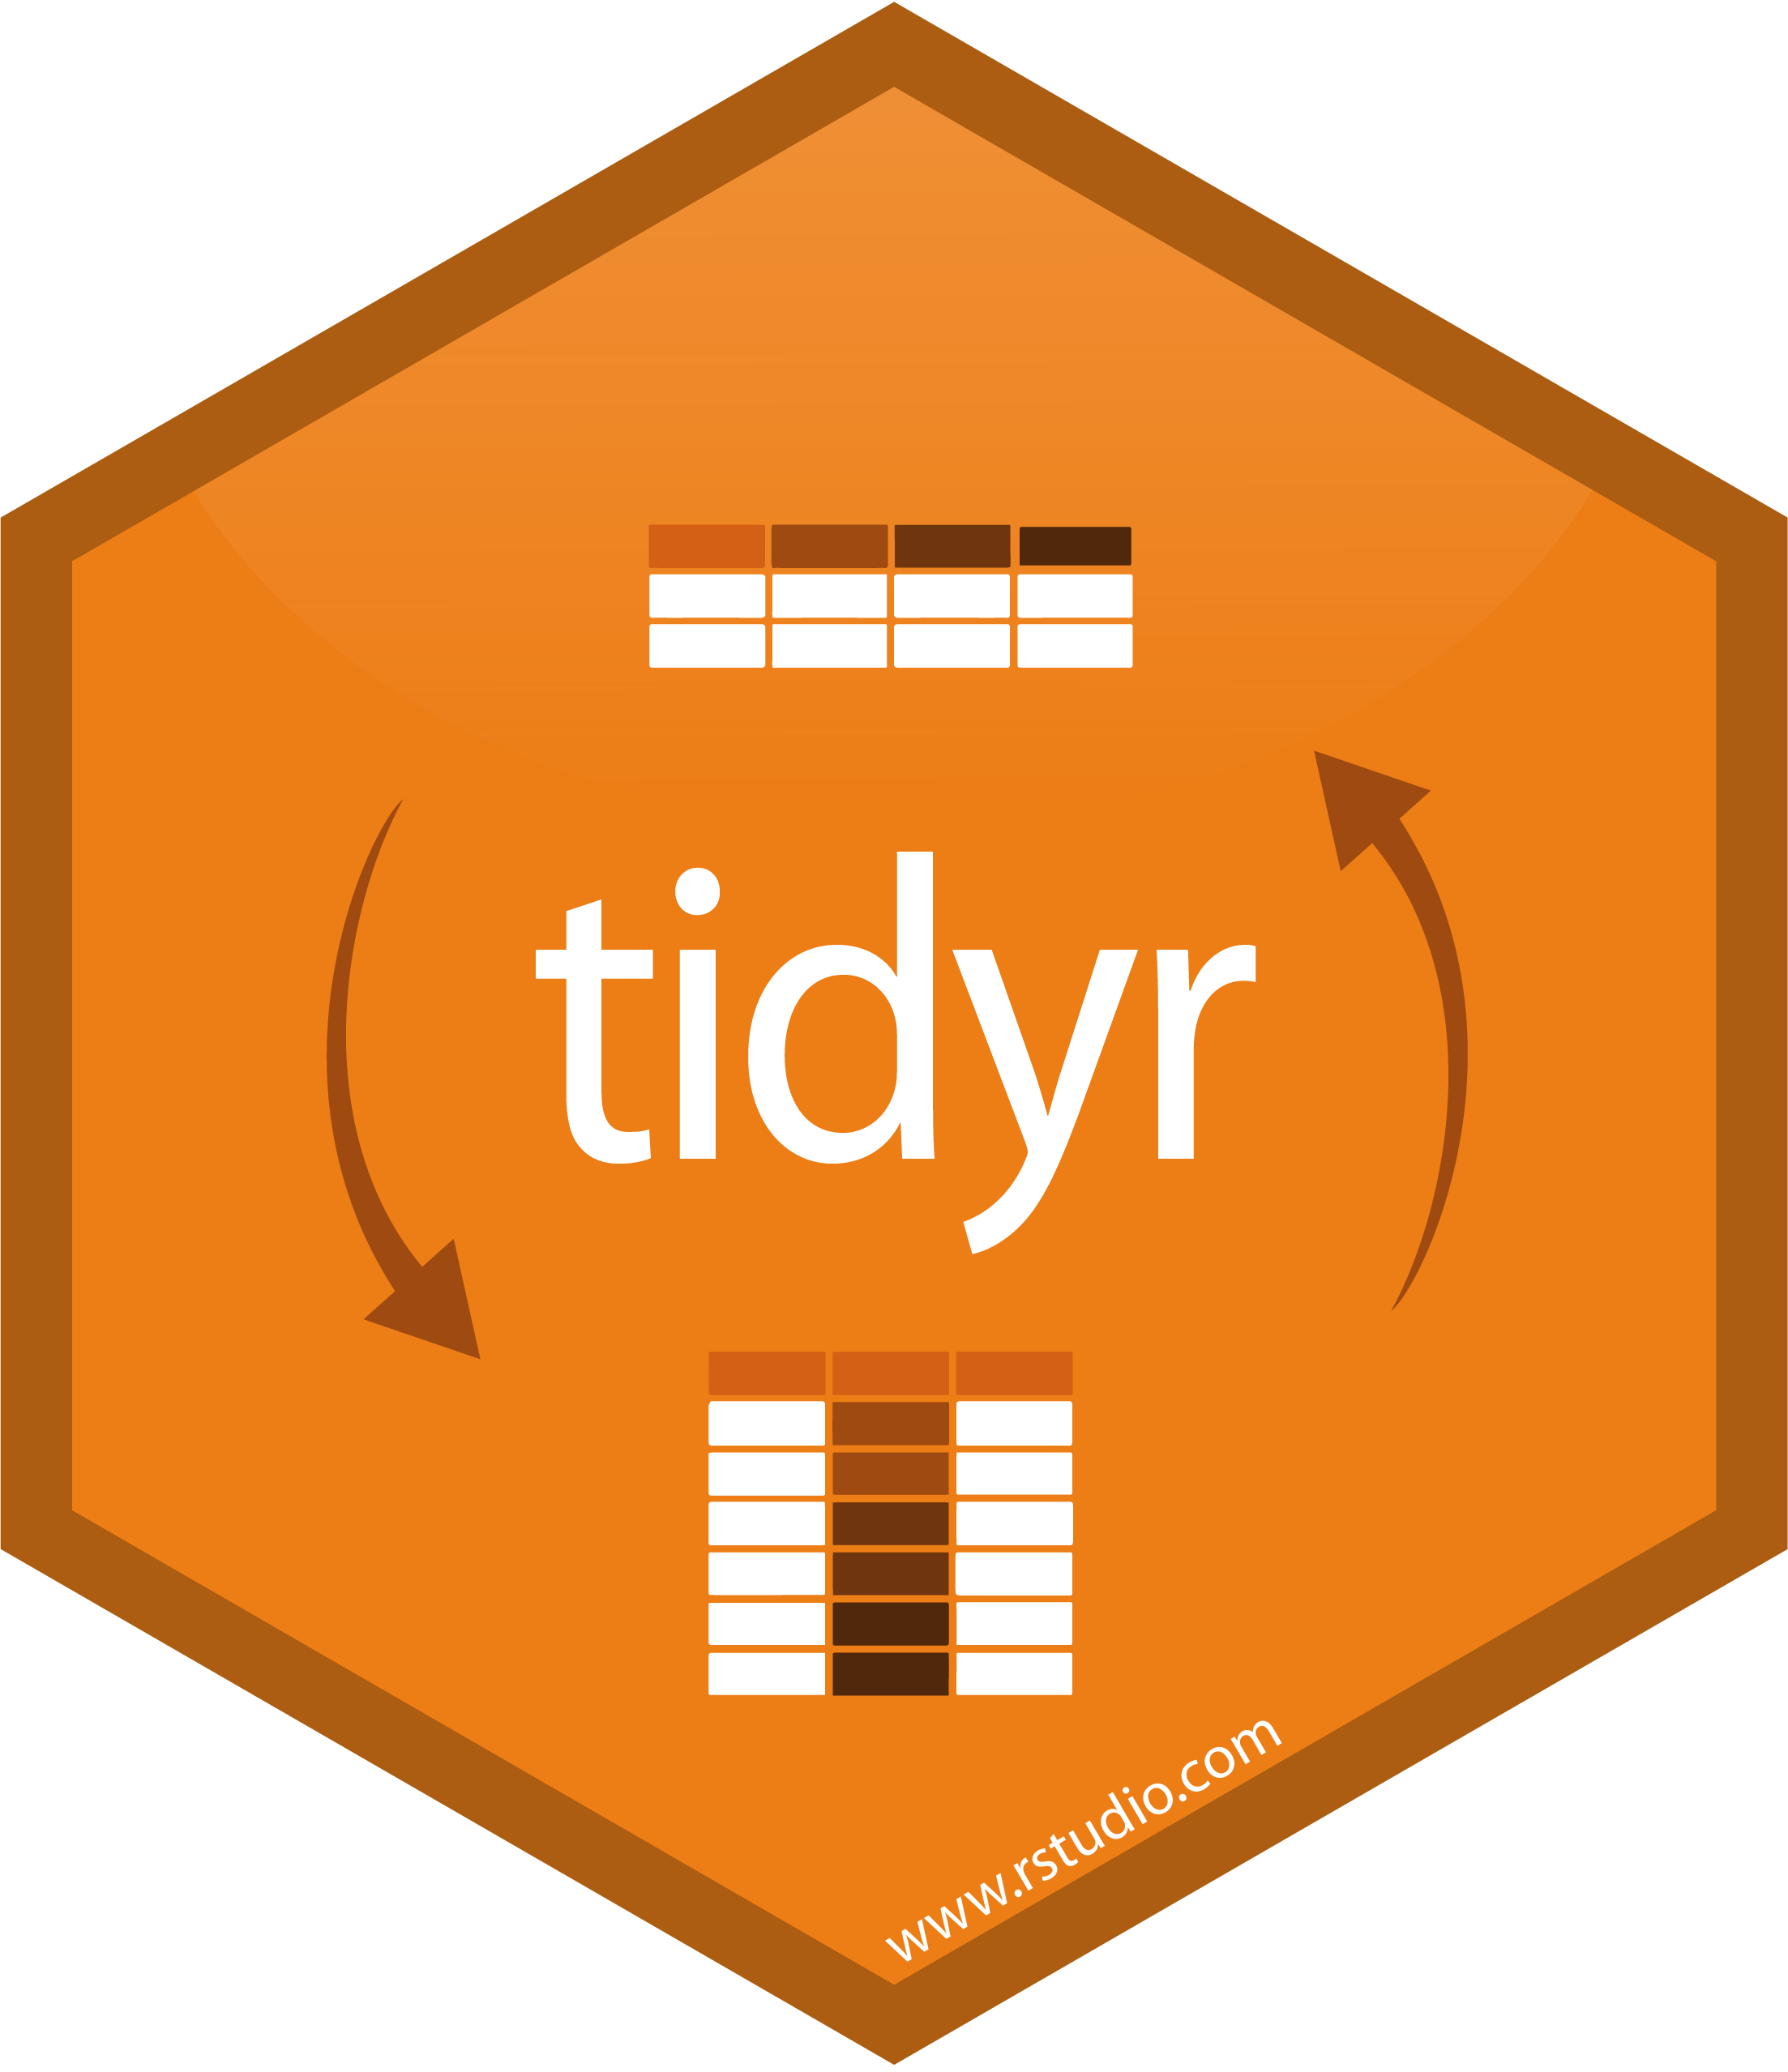
\includegraphics[width=1.5cm]{tidyr.png}
  };
\end{tikzpicture}

\begin{itemize}
\tightlist
\item
  O llevarla a un formato ancho
\end{itemize}

\begin{flushright}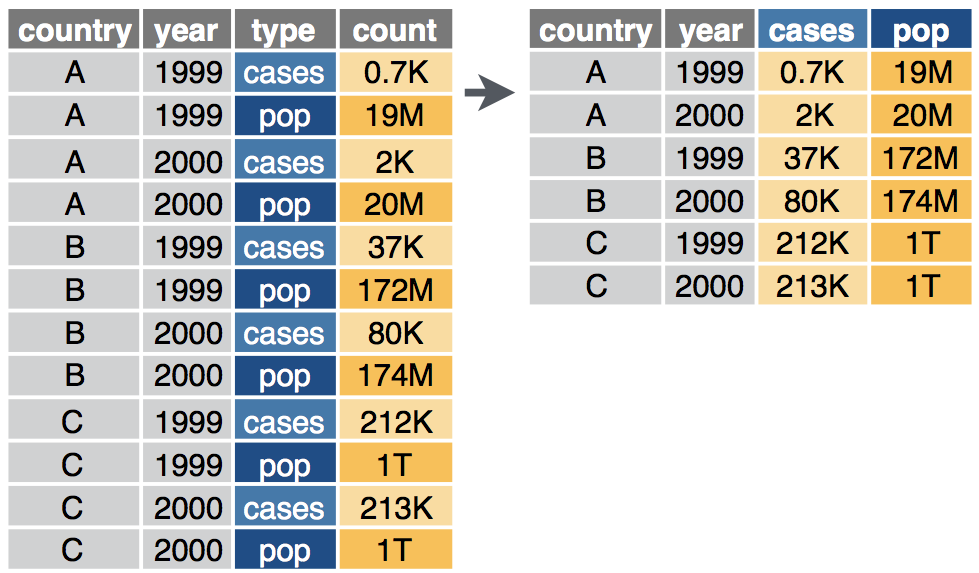
\includegraphics{pivot_wider_detailed} \end{flushright}

\end{frame}

\begin{frame}{}
\protect\hypertarget{section-7}{}

\begin{tikzpicture}[remember picture,overlay]
  \node[anchor=south west,inner sep=0pt] at ($(current page.south west)+(0cm,7.8cm)$) {
     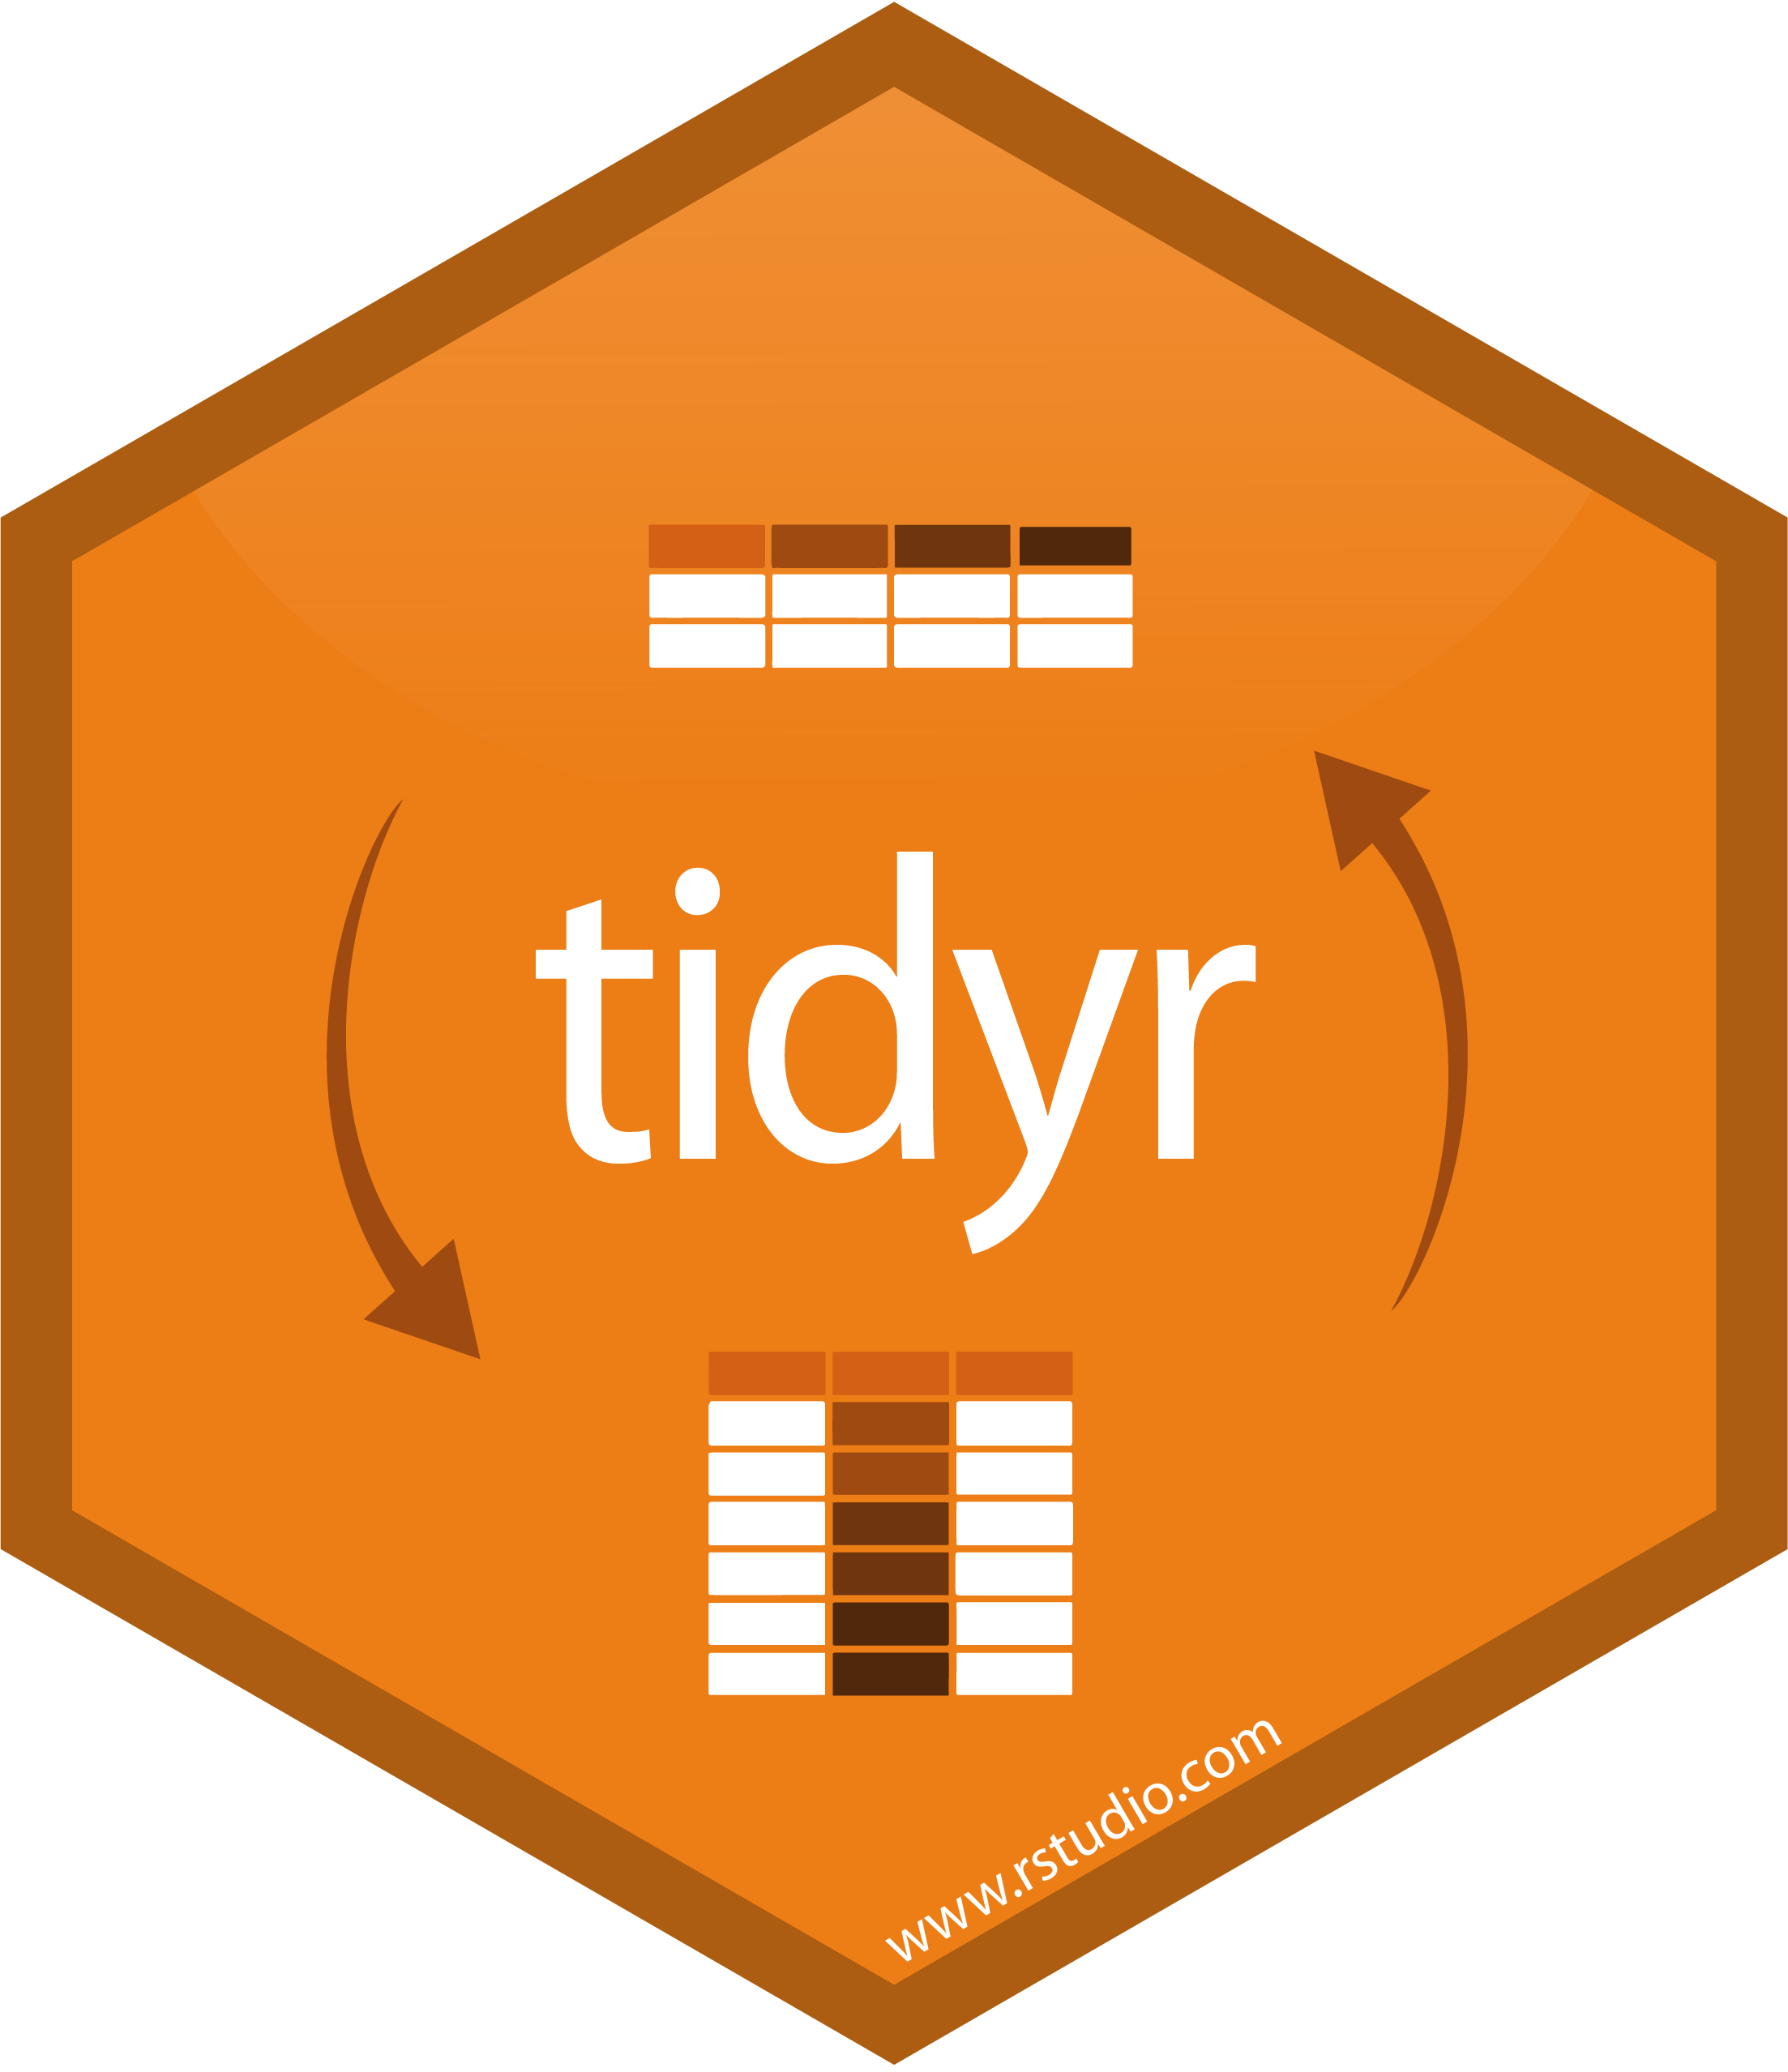
\includegraphics[width=1.5cm]{tidyr.png}
  };
\end{tikzpicture}

\begin{itemize}
\tightlist
\item
  Podemos separar valores en celdas
\end{itemize}

\begin{center}
\includegraphics[width=0.6\linewidth]{tidyr_separate} \end{center}

\begin{itemize}
\tightlist
\item
  O unirlos
\end{itemize}

\begin{center}
\includegraphics[width=0.6\linewidth]{tidyr_unite} \end{center}

\end{frame}

\begin{frame}{}
\protect\hypertarget{section-8}{}

\begin{tikzpicture}[remember picture,overlay]
  \node[anchor=south west,inner sep=0pt] at ($(current page.south west)+(0cm,7.8cm)$) {
     
\includegraphics[width=1.5cm]{ggplot2_logo.png}
  };
\end{tikzpicture}

\begin{itemize}
\tightlist
\item
  Es importante aca explicar cosas como lo de \textbf{aes()} y cosas del
  estilo. Para eso hay que leer bien un articulo sobre ggplot2!
\end{itemize}

\end{frame}

\begin{frame}{}
\protect\hypertarget{section-9}{}

\begin{tikzpicture}[remember picture,overlay]
  \node[anchor=south west,inner sep=0pt] at ($(current page.south west)+(0cm,7.8cm)$) {
     
\includegraphics[width=1.5cm]{ggplot2_logo.png}
  };
\end{tikzpicture}

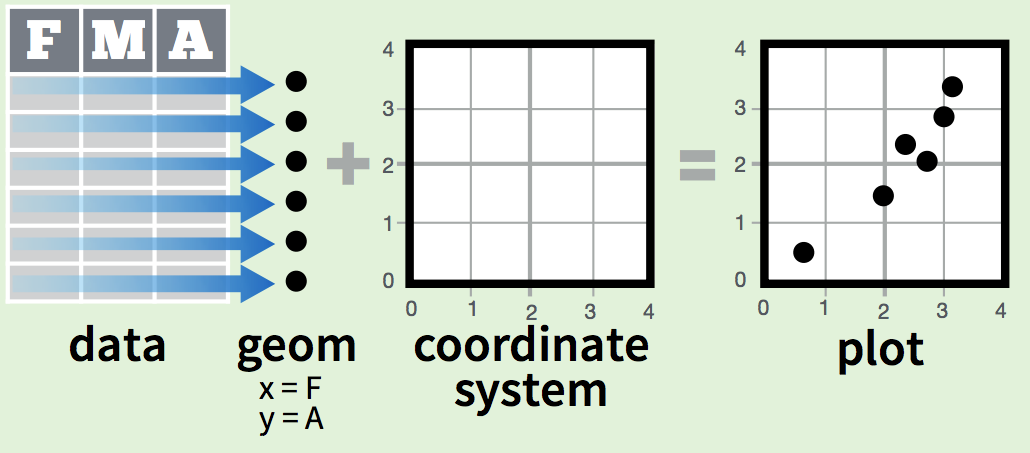
\includegraphics{ggplot_basico_1.png}

\end{frame}

\begin{frame}{}
\protect\hypertarget{section-10}{}

\begin{tikzpicture}[remember picture,overlay]
  \node[anchor=south west,inner sep=0pt] at ($(current page.south west)+(0cm,7.8cm)$) {
     
\includegraphics[width=1.5cm]{ggplot2_logo.png}
  };
\end{tikzpicture}

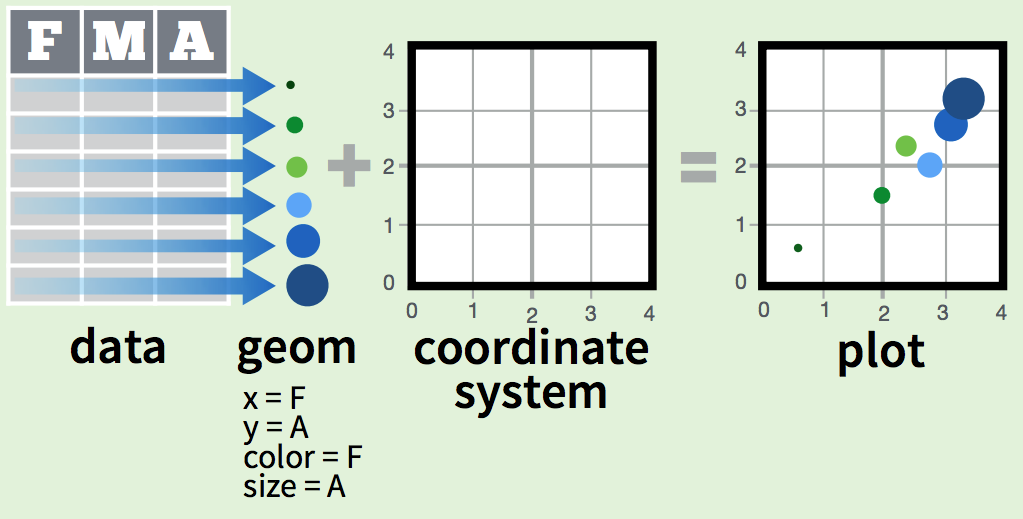
\includegraphics{ggplot_basico_2.png}

\end{frame}

\begin{frame}[fragile]{}
\protect\hypertarget{section-11}{}

\begin{tikzpicture}[remember picture,overlay]
  \node[anchor=south west,inner sep=0pt] at ($(current page.south west)+(0cm,7.8cm)$) {
     
\includegraphics[width=1.5cm]{ggplot2_logo.png}
  };
\end{tikzpicture}

\begin{Shaded}
\begin{Highlighting}[]
\KeywordTok{library}\NormalTok{(tidyverse)}
  \CommentTok{# se grafica Sepal.Length vs Sepal.Width,}
  \CommentTok{# coloreando segun Species}
\KeywordTok{ggplot}\NormalTok{(}\DataTypeTok{data =}\NormalTok{ iris,}
          \KeywordTok{aes}\NormalTok{(}\DataTypeTok{x =}\NormalTok{ Sepal.Length, }
              \DataTypeTok{y =}\NormalTok{ Sepal.Width, }
              \DataTypeTok{color =}\NormalTok{ Species, }
              \DataTypeTok{fill =}\NormalTok{ Species)) }\OperatorTok{+}
\StringTok{  }\CommentTok{# se grafica utilizando puntos}
\StringTok{  }\KeywordTok{geom_point}\NormalTok{() }
\end{Highlighting}
\end{Shaded}

\end{frame}

\begin{frame}{}
\protect\hypertarget{section-12}{}

\begin{tikzpicture}[remember picture,overlay]
  \node[anchor=south west,inner sep=0pt] at ($(current page.south west)+(0cm,7.8cm)$) {
     
\includegraphics[width=1.5cm]{ggplot2_logo.png}
  };
\end{tikzpicture}

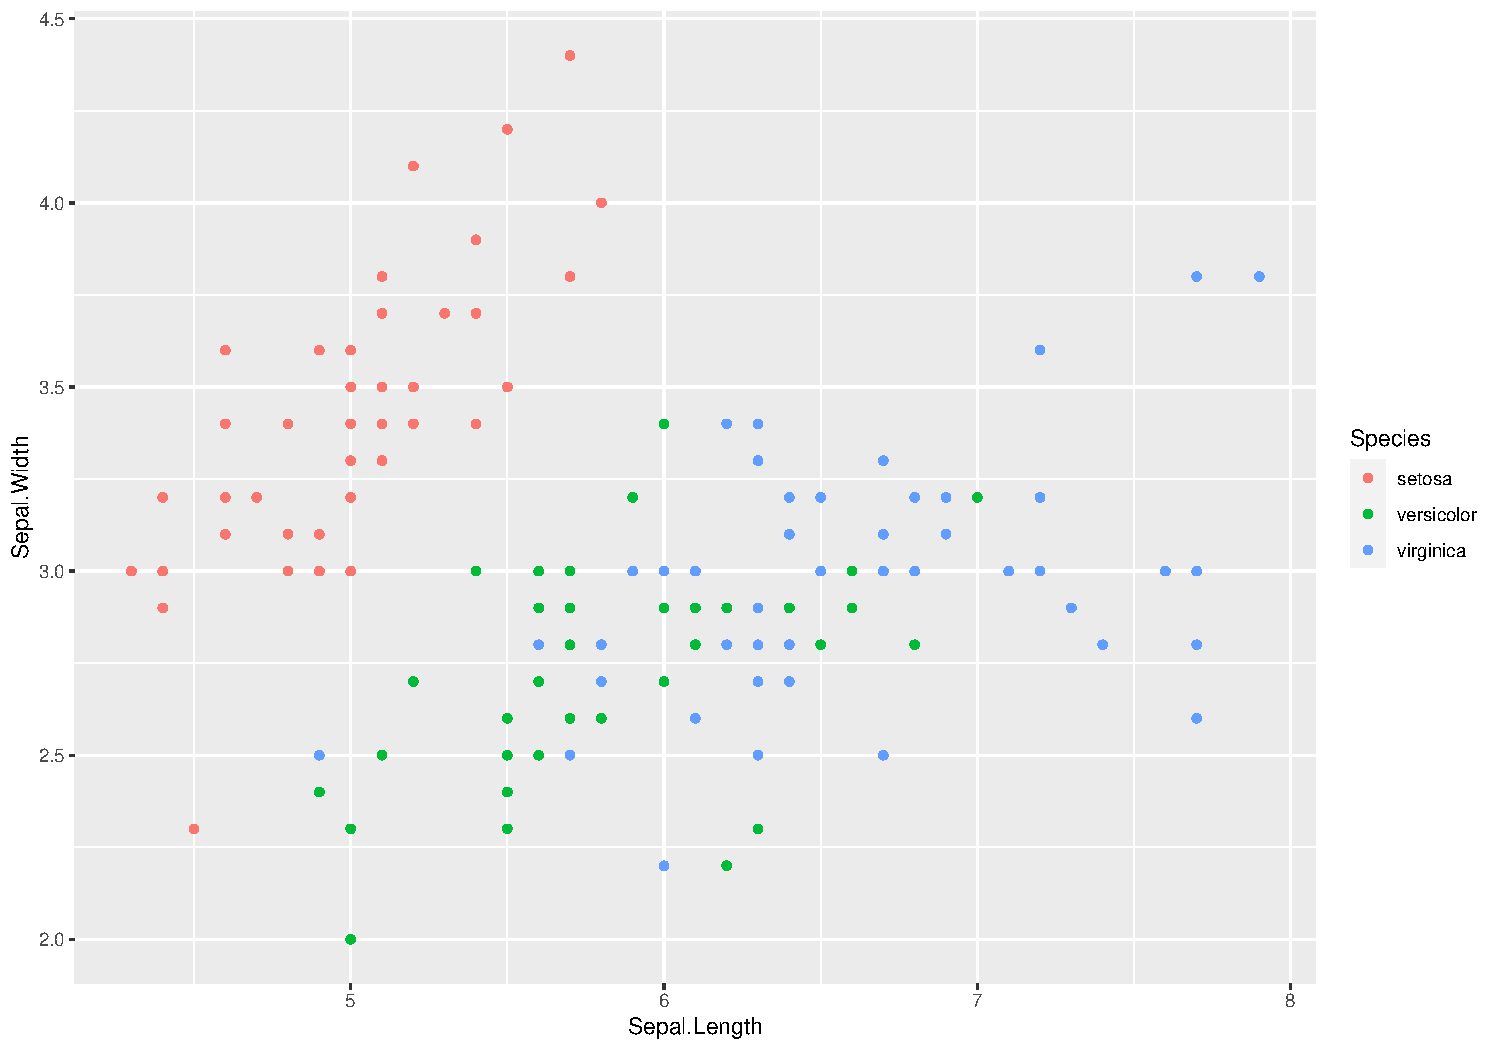
\includegraphics{claseIntro_practico12_final_files/figure-beamer/unnamed-chunk-26-1.pdf}

\end{frame}

\begin{frame}{}
\protect\hypertarget{section-13}{}


\includegraphics{streamlining-with-magrittr.jpg}

\end{frame}

\begin{frame}{}
\protect\hypertarget{section-14}{}

\begin{tikzpicture}[remember picture,overlay]
  \node[anchor=south west,inner sep=0pt] at ($(current page.south west)+(0cm,7.8cm)$) {
     
\includegraphics[width=1.5cm]{magrittr_log.jpg}
  };
\end{tikzpicture}

\begin{itemize}
\tightlist
\item
  Es el \emph{pipe} de R.
\item
  El uso es exactamente igual al `\textbar{}' de Bash.
\item
  Un único detalle: se utiliza \textbf{.} para hacer referencia a
  resultados intermedios en un pipe.
\end{itemize}

\end{frame}

\begin{frame}[fragile]{}
\protect\hypertarget{section-15}{}

\begin{tikzpicture}[remember picture,overlay]
  \node[anchor=south west,inner sep=0pt] at ($(current page.south west)+(0cm,7.8cm)$) {
     
\includegraphics[width=1.5cm]{magrittr_log.jpg}
  };
\end{tikzpicture}

\begin{Shaded}
\begin{Highlighting}[]
\CommentTok{# con magrittr}
\KeywordTok{library}\NormalTok{(magrittr)}

\NormalTok{Sepal.Width.Median =}\StringTok{ }\NormalTok{iris }\OperatorTok\StringTok{ }\NormalTok{.}\OperatorTok{$}\NormalTok{Sepal.Width }\OperatorTok\StringTok{ }\KeywordTok{median}\NormalTok{(.) }
\end{Highlighting}
\end{Shaded}

\end{frame}

\begin{frame}{¿Donde encuentro info sobre estos paquetes?}
\protect\hypertarget{donde-encuentro-info-sobre-estos-paquetes}{}

\begin{itemize}
\tightlist
\item
  Cheatsheets
\item
  Vignettes
\end{itemize}

\end{frame}

\begin{frame}{¿Donde encuentro info sobre estos paquetes?}
\protect\hypertarget{donde-encuentro-info-sobre-estos-paquetes-1}{}

\begin{center}
\includegraphics[width=0.45\linewidth]{cover_rfordatascience} \end{center}

\end{frame}

\hypertarget{bonus}{%
\section{Bonus}\label{bonus}}

\begin{frame}{GGally: análisis exploratorios y otros}
\protect\hypertarget{ggally-anuxe1lisis-exploratorios-y-otros}{}

\small

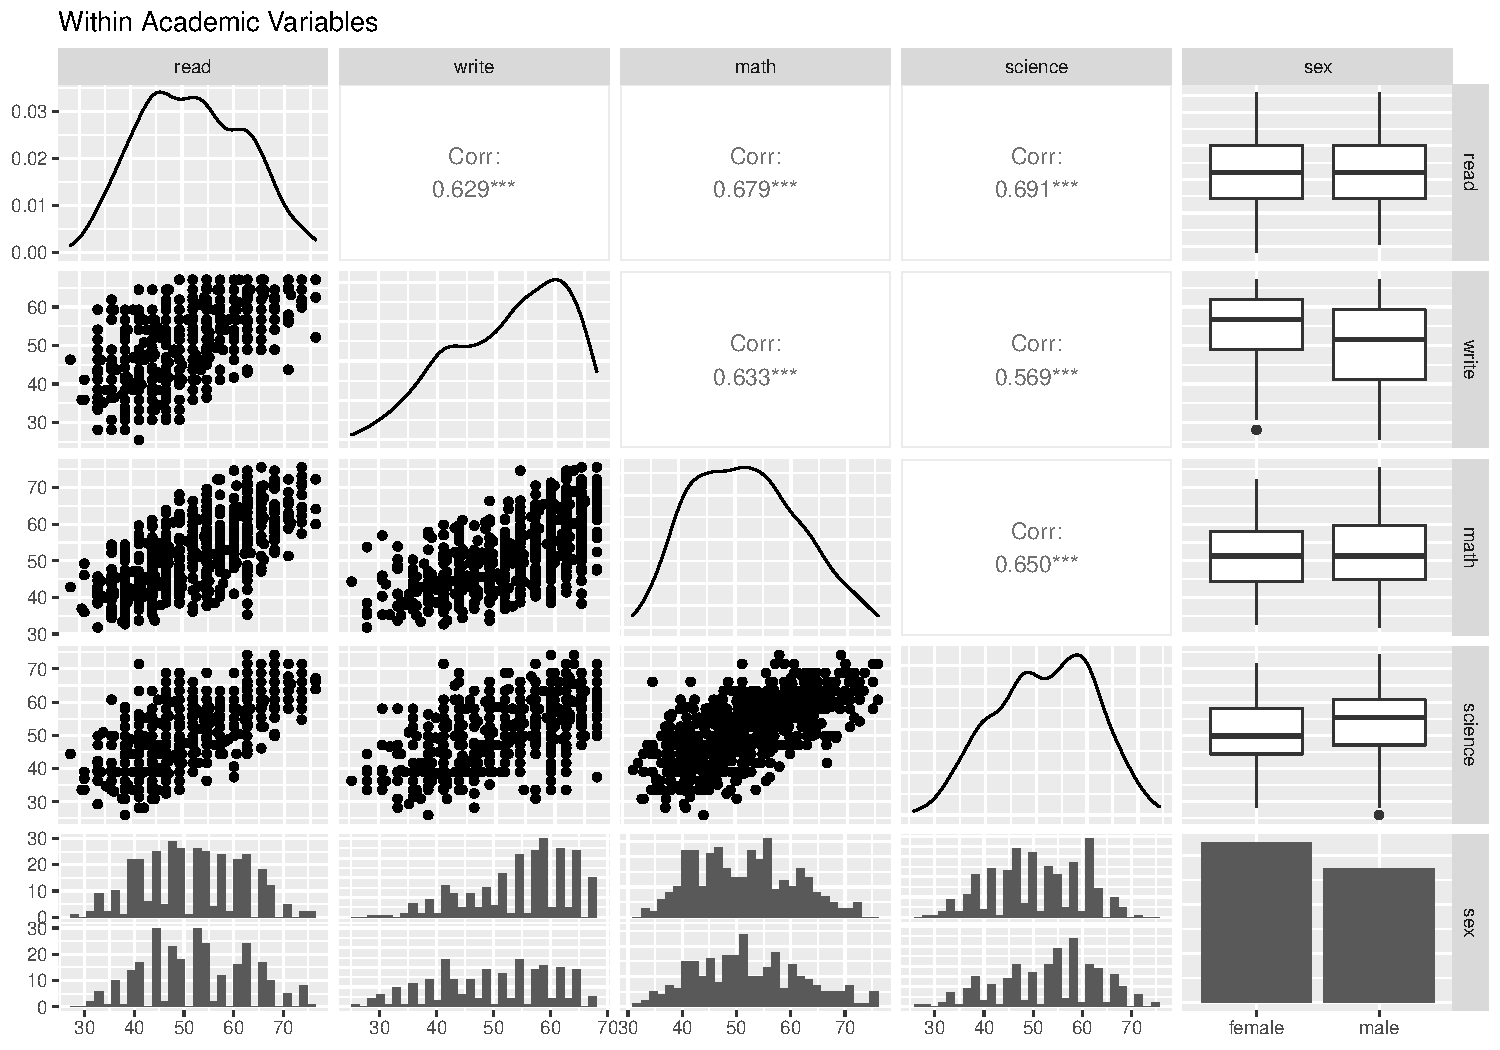
\includegraphics{claseIntro_practico12_final_files/figure-beamer/unnamed-chunk-31-1.pdf}

\normalsize

\end{frame}

\begin{frame}{Filogenética: librería ggtree}
\protect\hypertarget{filogenuxe9tica-libreruxeda-ggtree}{}

\small

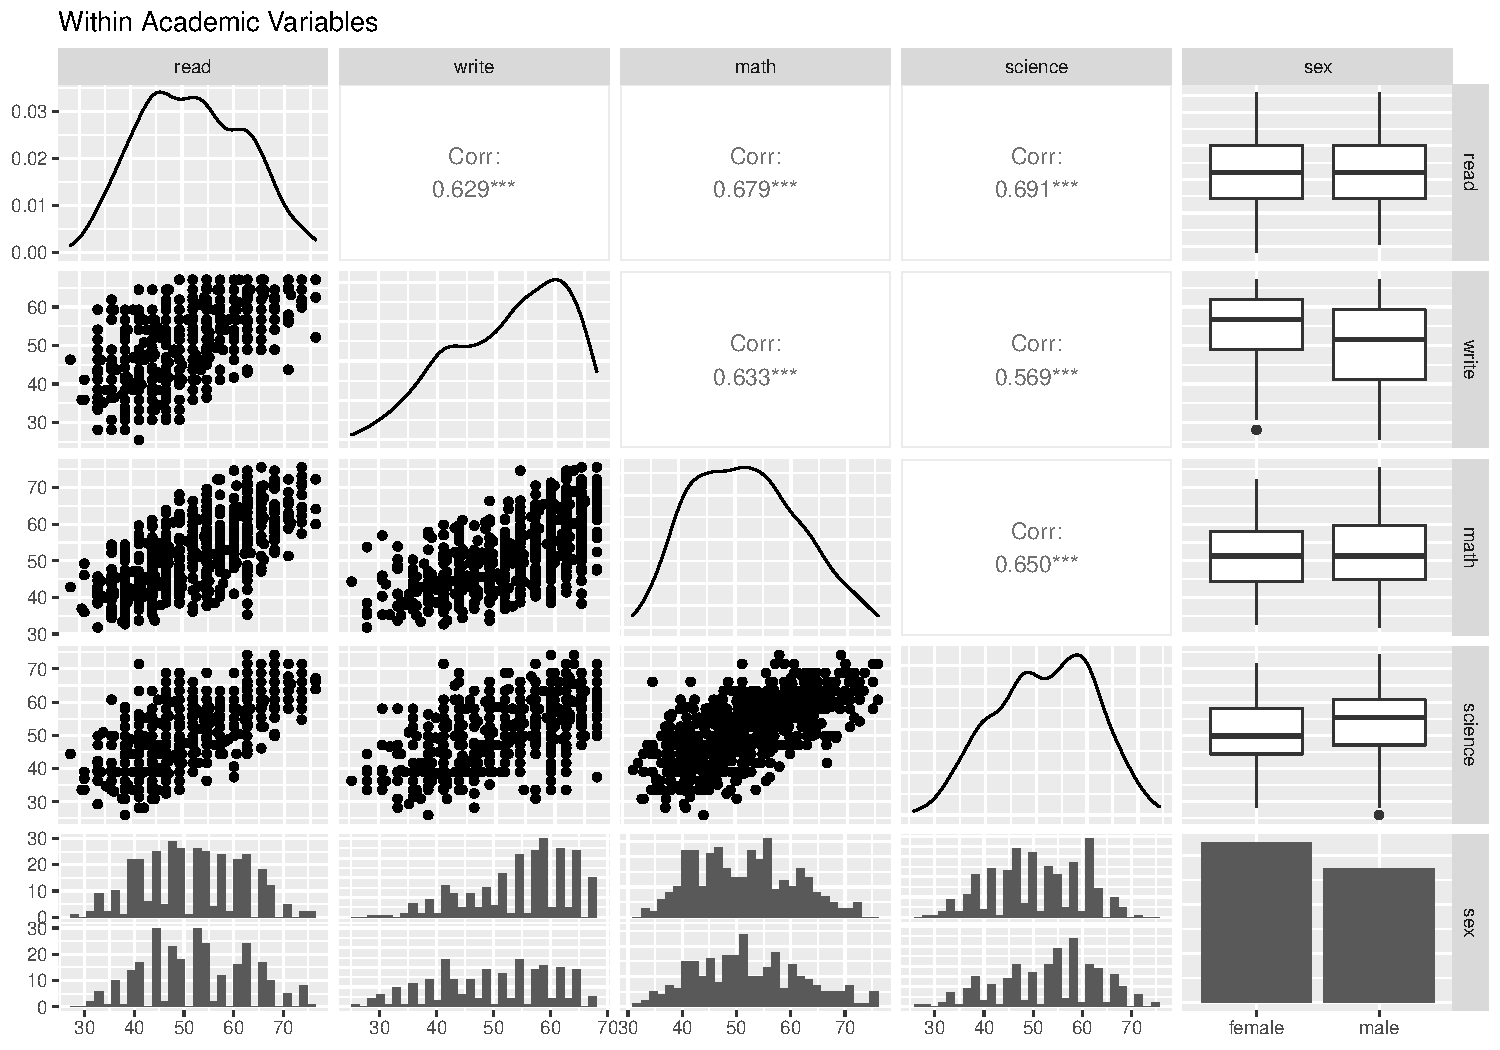
\includegraphics{claseIntro_practico12_final_files/figure-beamer/unnamed-chunk-32-1.pdf}

\normalsize

\end{frame}

\begin{frame}{Genómica: BioCircos/\textbf{rcirclize} y gggnomics, ggbio}
\protect\hypertarget{genuxf3mica-biocircosrcirclize-y-gggnomics-ggbio}{}

\begin{center}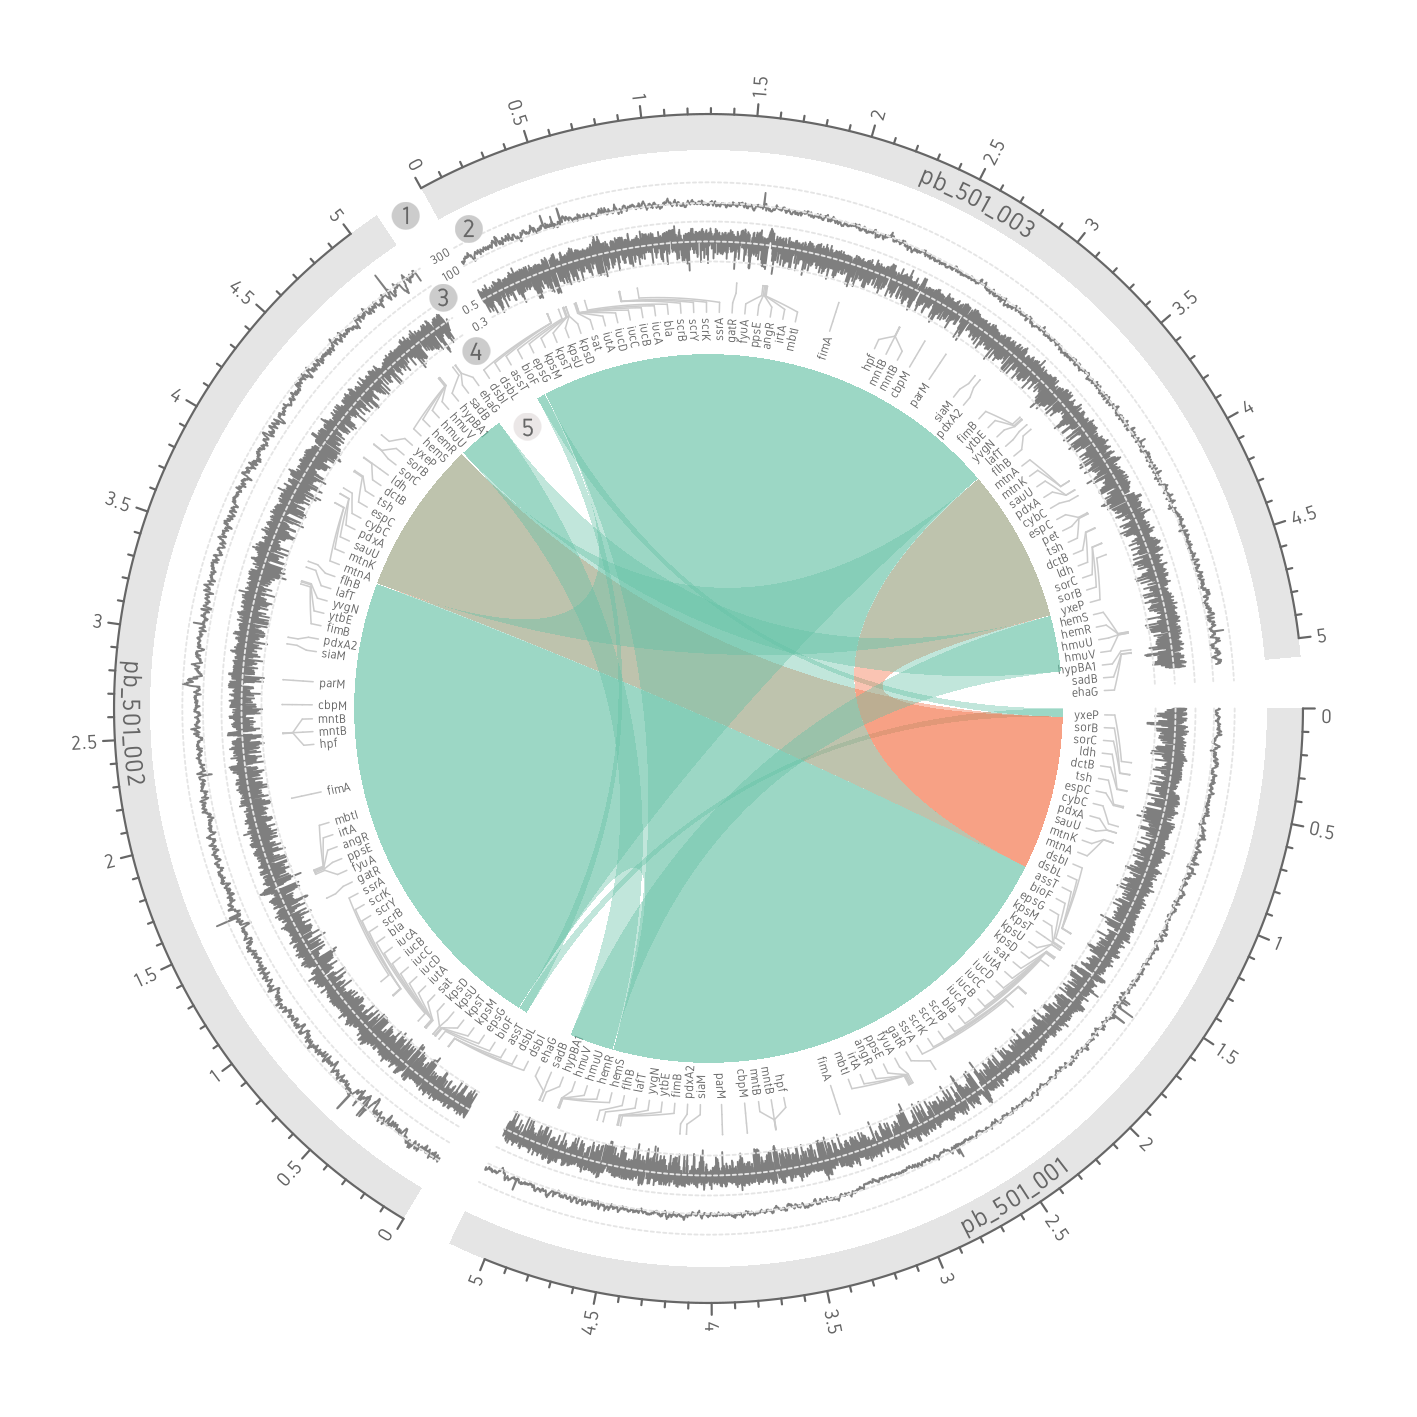
\includegraphics[width=0.95\linewidth]{rcirclize} \end{center}

\end{frame}

\begin{frame}{Genómica: BioCircos/rcirclize y gggnomics, \textbf{ggbio}}
\protect\hypertarget{genuxf3mica-biocircosrcirclize-y-gggnomics-ggbio-1}{}

\begin{center}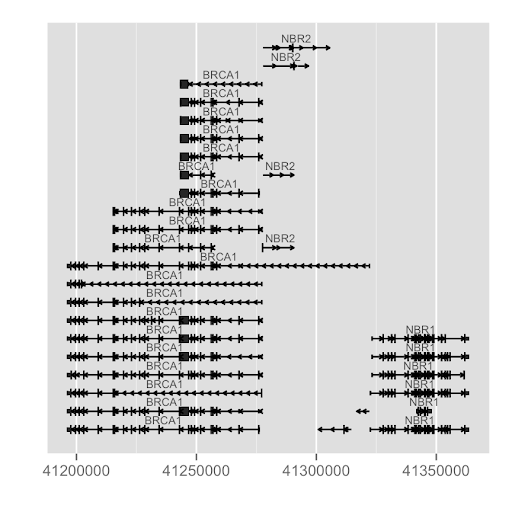
\includegraphics[width=0.95\linewidth]{ggnomics_1} \end{center}

\end{frame}

\begin{frame}{Genómica: BioCircos/rcirclize y gggnomics, \textbf{ggbio}}
\protect\hypertarget{genuxf3mica-biocircosrcirclize-y-gggnomics-ggbio-2}{}

\begin{center}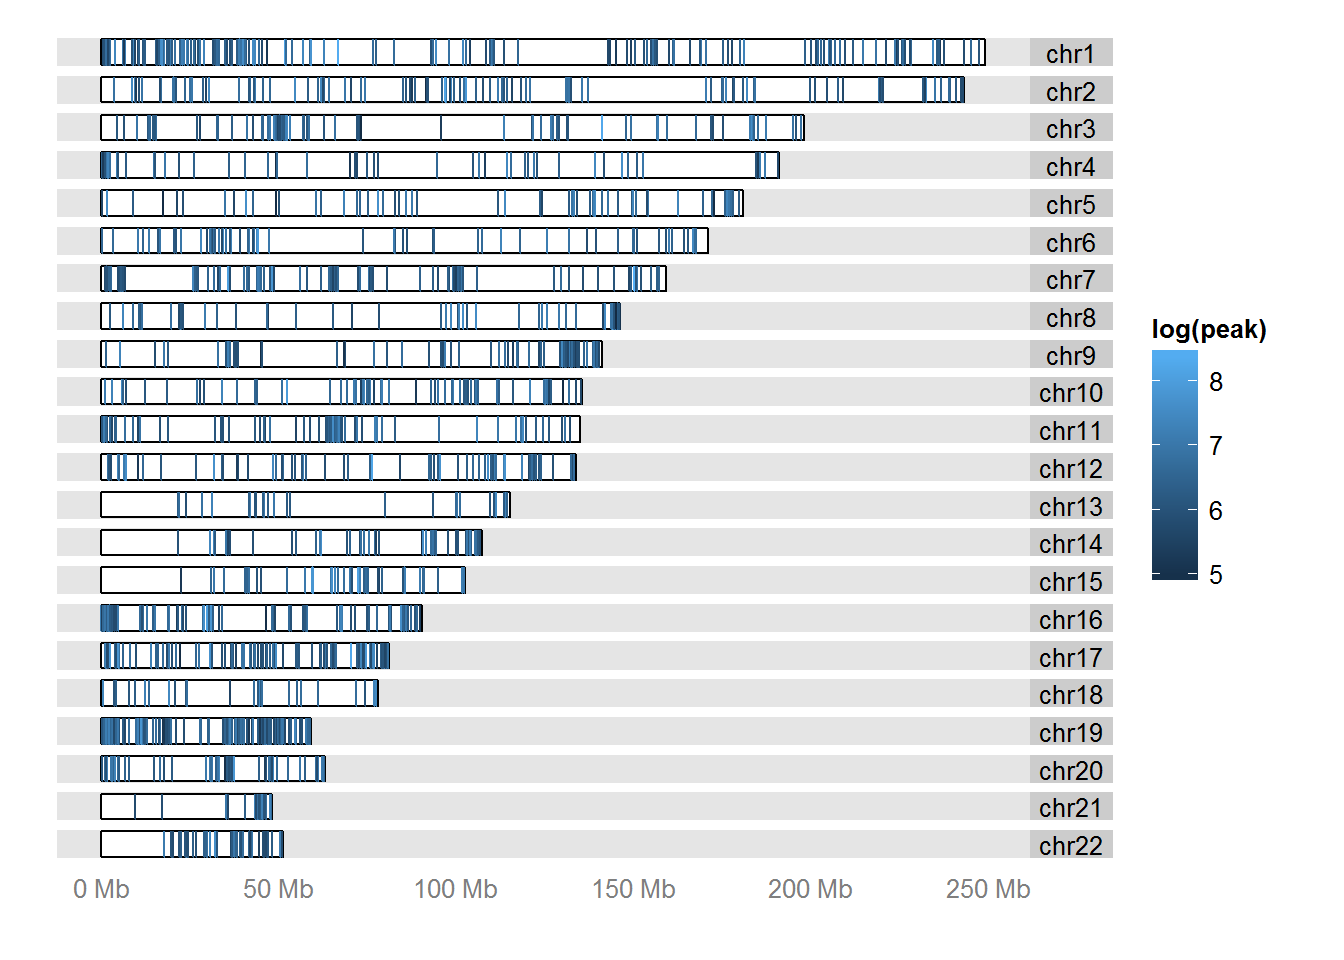
\includegraphics[width=0.95\linewidth]{ggnomics_2} \end{center}

\end{frame}

\end{document}
